
% ════════════════════════════════════════════
% 数据清洗与特征整理（5.2）
% ════════════════════════════════════════════
\subsection{数据清洗与特征整理}

\subsubsection{缺失、异常与编码}

原始数据只有 1 条缺失、0 条重复，但类别变量的稀疏程度与因变量的重尾程度都超出线性回归的适用条件。付费标记 X7 仅在编号 499 的帖子缺失，占 0.2\%，该帖其余字段完整，删除会浪费一条有效信息，故采用众数填补，取值为 0，并附加填补标记以便追溯。7 个输入变量的取值范围全部落在字段说明之内，没有越界值；X6 的 0 时与 21 时没有帖子，实际只有 22 个取值；Y1 的 1,110,282 次是一条真实的病毒式传播记录，不作删除，改由 log1p 变换压缩其影响。

编码遵循“$K$ 个水平保留 $K-1$ 个哑变量”的规则。帖子类型以 Photo 为参照，保留 Status、Link、Video 三个哑变量；内容主题以主题 1 为参照，保留主题 2、主题 3 两个哑变量；月份与星期分别生成 11 个和 6 个哑变量，参照类为 1 月与周一；发帖小时合并为凌晨（0 至 5 时）、上午（6 至 11 时）与下午晚间（12 至 23 时）三组，并以上午为参照，三组分别有 196、193、111 条，均超过 100 条。加上常数项与付费标记，最终模型共需 $1+3+2+11+6+2+1=26$ 个参数。

图\ref{fig:q2_cat}显示，Photo 有 426 条，占 85.2\%，Status 45 条、Link 22 条、Video 仅 7 条；三类主题分别为 215、130、155 条，相对均衡；付费标记在填补后为自然 361 条、付费 139 条；发帖小时呈双峰分布，凌晨 3 时最多（105 条），上午 10 时次之（78 条）。视频与链接的样本量提示其估计精度有限，这一限制将在效应区间中直接体现。

\begin{figure}[ht]
  \centering
  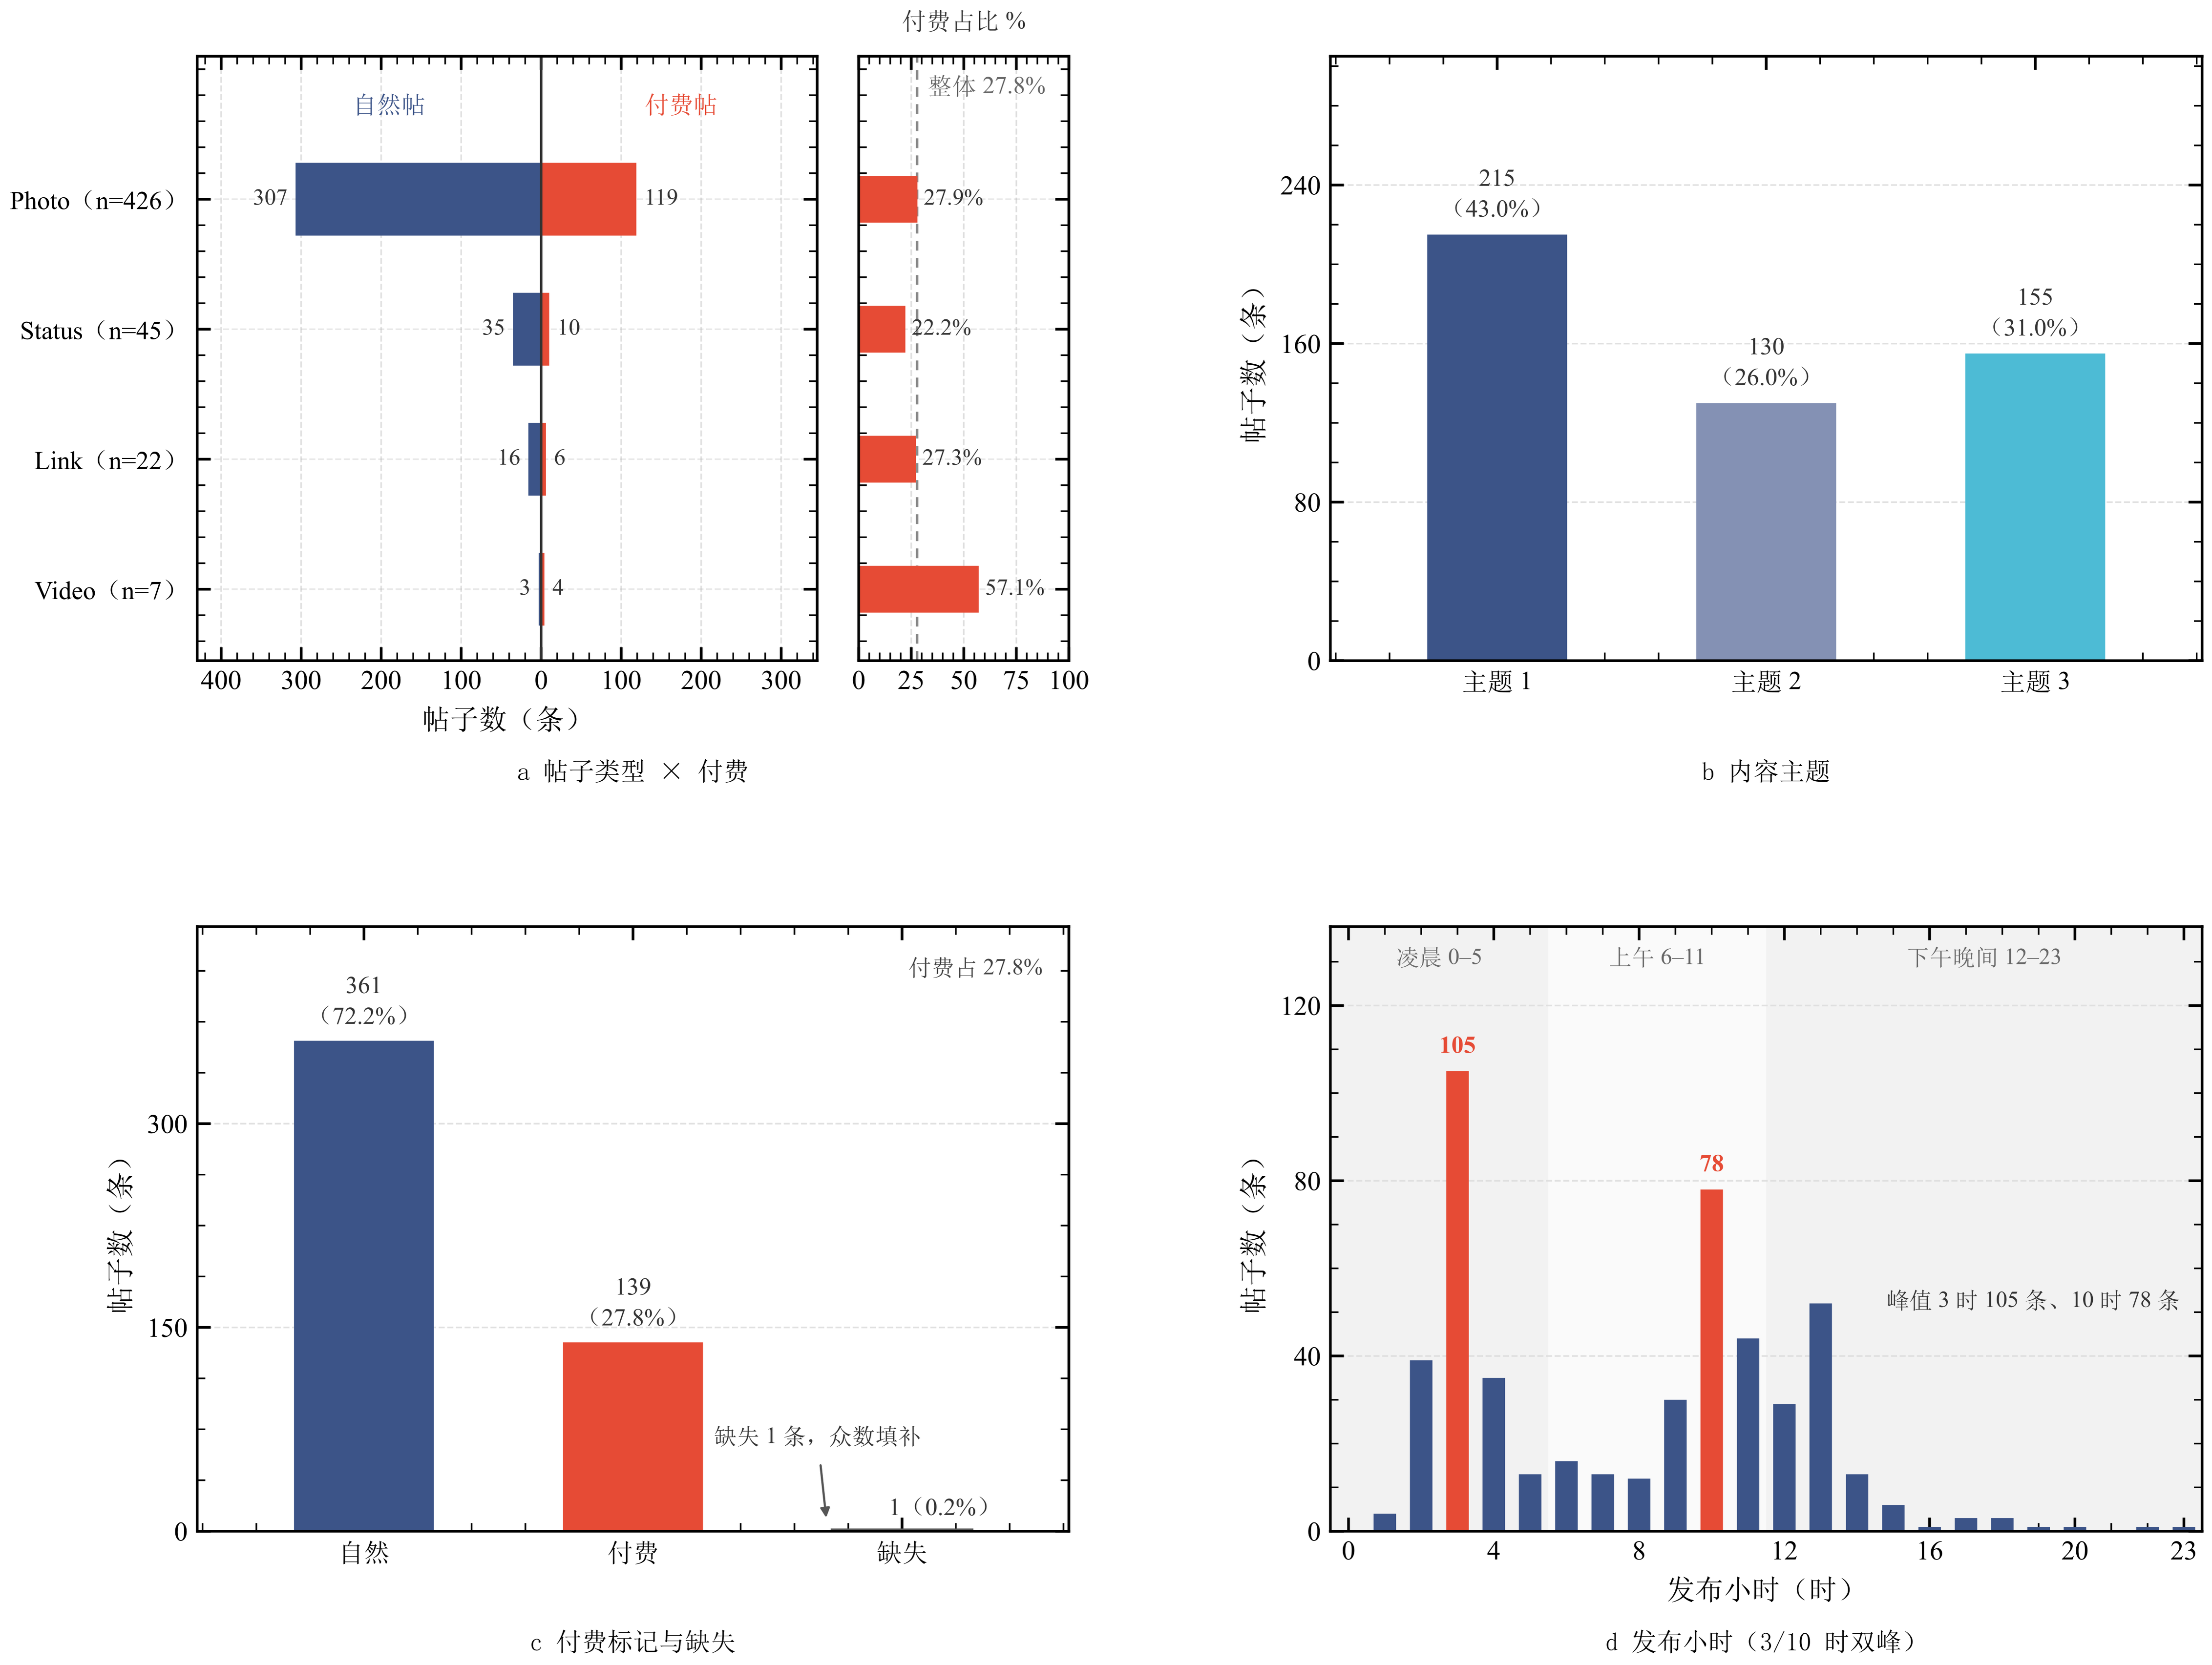
\includegraphics[width=0.70\textwidth]{../求解/问题二/结果/图4_类别结构与缺失.png}
  \caption{类别结构与缺失分布}
  \label{fig:q2_cat}
\end{figure}

表\ref{tab:q2_scheme}汇总了编码与变换方案。连续变量 X1 取对数，计数型因变量 Y1 取 log1p；名义变量 X2、X3 分别以 Photo、主题 1 为参照；月份、星期保留全部哑变量；时段合并为三组；X7 保持 0/1 数值。该方案共产生 26 个参数，与最终回归模型一致。

\begin{longtable}{>{\centering\arraybackslash}p{0.10\textwidth}>{\centering\arraybackslash}p{0.14\textwidth}>{\centering\arraybackslash}p{0.20\textwidth}>{\centering\arraybackslash}p{0.14\textwidth}>{\centering\arraybackslash}p{0.26\textwidth}}
  \caption{编码与变换方案}
  \label{tab:q2_scheme} \\
  \toprule
  变量 & 识别类型 & 编码或变换 & 基线或参照 & 解释 \\
  \midrule
  \endfirsthead
  \caption{编码与变换方案（续）} \\
  \toprule
  变量 & 识别类型 & 编码或变换 & 基线或参照 & 解释 \\
  \midrule
  \endhead
  \bottomrule
  \endfoot
  X1 & 连续 & $\log(X_1)$ & 无 & 粉丝规模弹性，压缩量级 \\
  X2 & 名义，4 类 & 独热编码，3 个哑变量 & Photo & 相对图片的曝光差异 \\
  X3 & 名义，3 类 & 独热编码，2 个哑变量 & 主题 1 & 相对主题 1 的曝光差异 \\
  X4 & 有序，12 类 & 独热编码，11 个哑变量 & 1 月 & 控制季节性与时间趋势 \\
  X5 & 有序，7 类 & 独热编码，6 个哑变量 & 周一 & 控制星期效应 \\
  X6 & 有序，24 类 & 合并 3 组，2 个哑变量 & 上午 & 控制时段效应，避免稀疏 \\
  X7 & 二元 & 0/1 数值 & 0，自然 & 付费的额外曝光 \\
  Y1 & 连续计数 & $\log(1+Y_1)$ & 无 & 压缩重尾，系数近似百分比 \\
\end{longtable}

\subsubsection{变换与敏感性}

曝光量为非负计数且右偏严重，采用 log1p 变换，即对曝光次数加 1 后取自然对数；加 1 保证曝光为零时有定义，本样本最小值为 570，实际不受影响。粉丝规模采用对数变换，把“每增加一人”改为“每增加 1\%”的弹性口径。两处变换只改变尺度，不改变样本排序。曝光量偏度由 8.3259 降至 0.7341，峰度由 93.0526 降至 0.8209，两项指标都回到接近正态的范围；最小值与最大值保持不变，说明变换没有删改任何观测。粉丝规模取对数后偏度由 $-0.9795$ 变为 $-1.1541$，左偏略有加强，这是粉丝数在高位堆积的必然结果，但其量级跨度被显著压缩，有利于数值稳定。

图\ref{fig:q2_trans}从分布形态与分位数两个角度对比变换效果。原始曝光量的直方图在 38 个等宽区间内有 396 条帖子落入首个区间，占 79.2\%；改用 30 个区间时为 414 条，占 82.8\%，两种分箱口径都显示首箱高度集中，其余观测拖出长尾。log1p 变换后的密度曲线与正态密度接近重合，Q--Q 图上的点也基本沿参考线分布，仅两端略有偏离。这说明 log1p 既保留了样本排序，又把极端值拉回了可建模的范围。

\begin{figure}[ht]
  \centering
  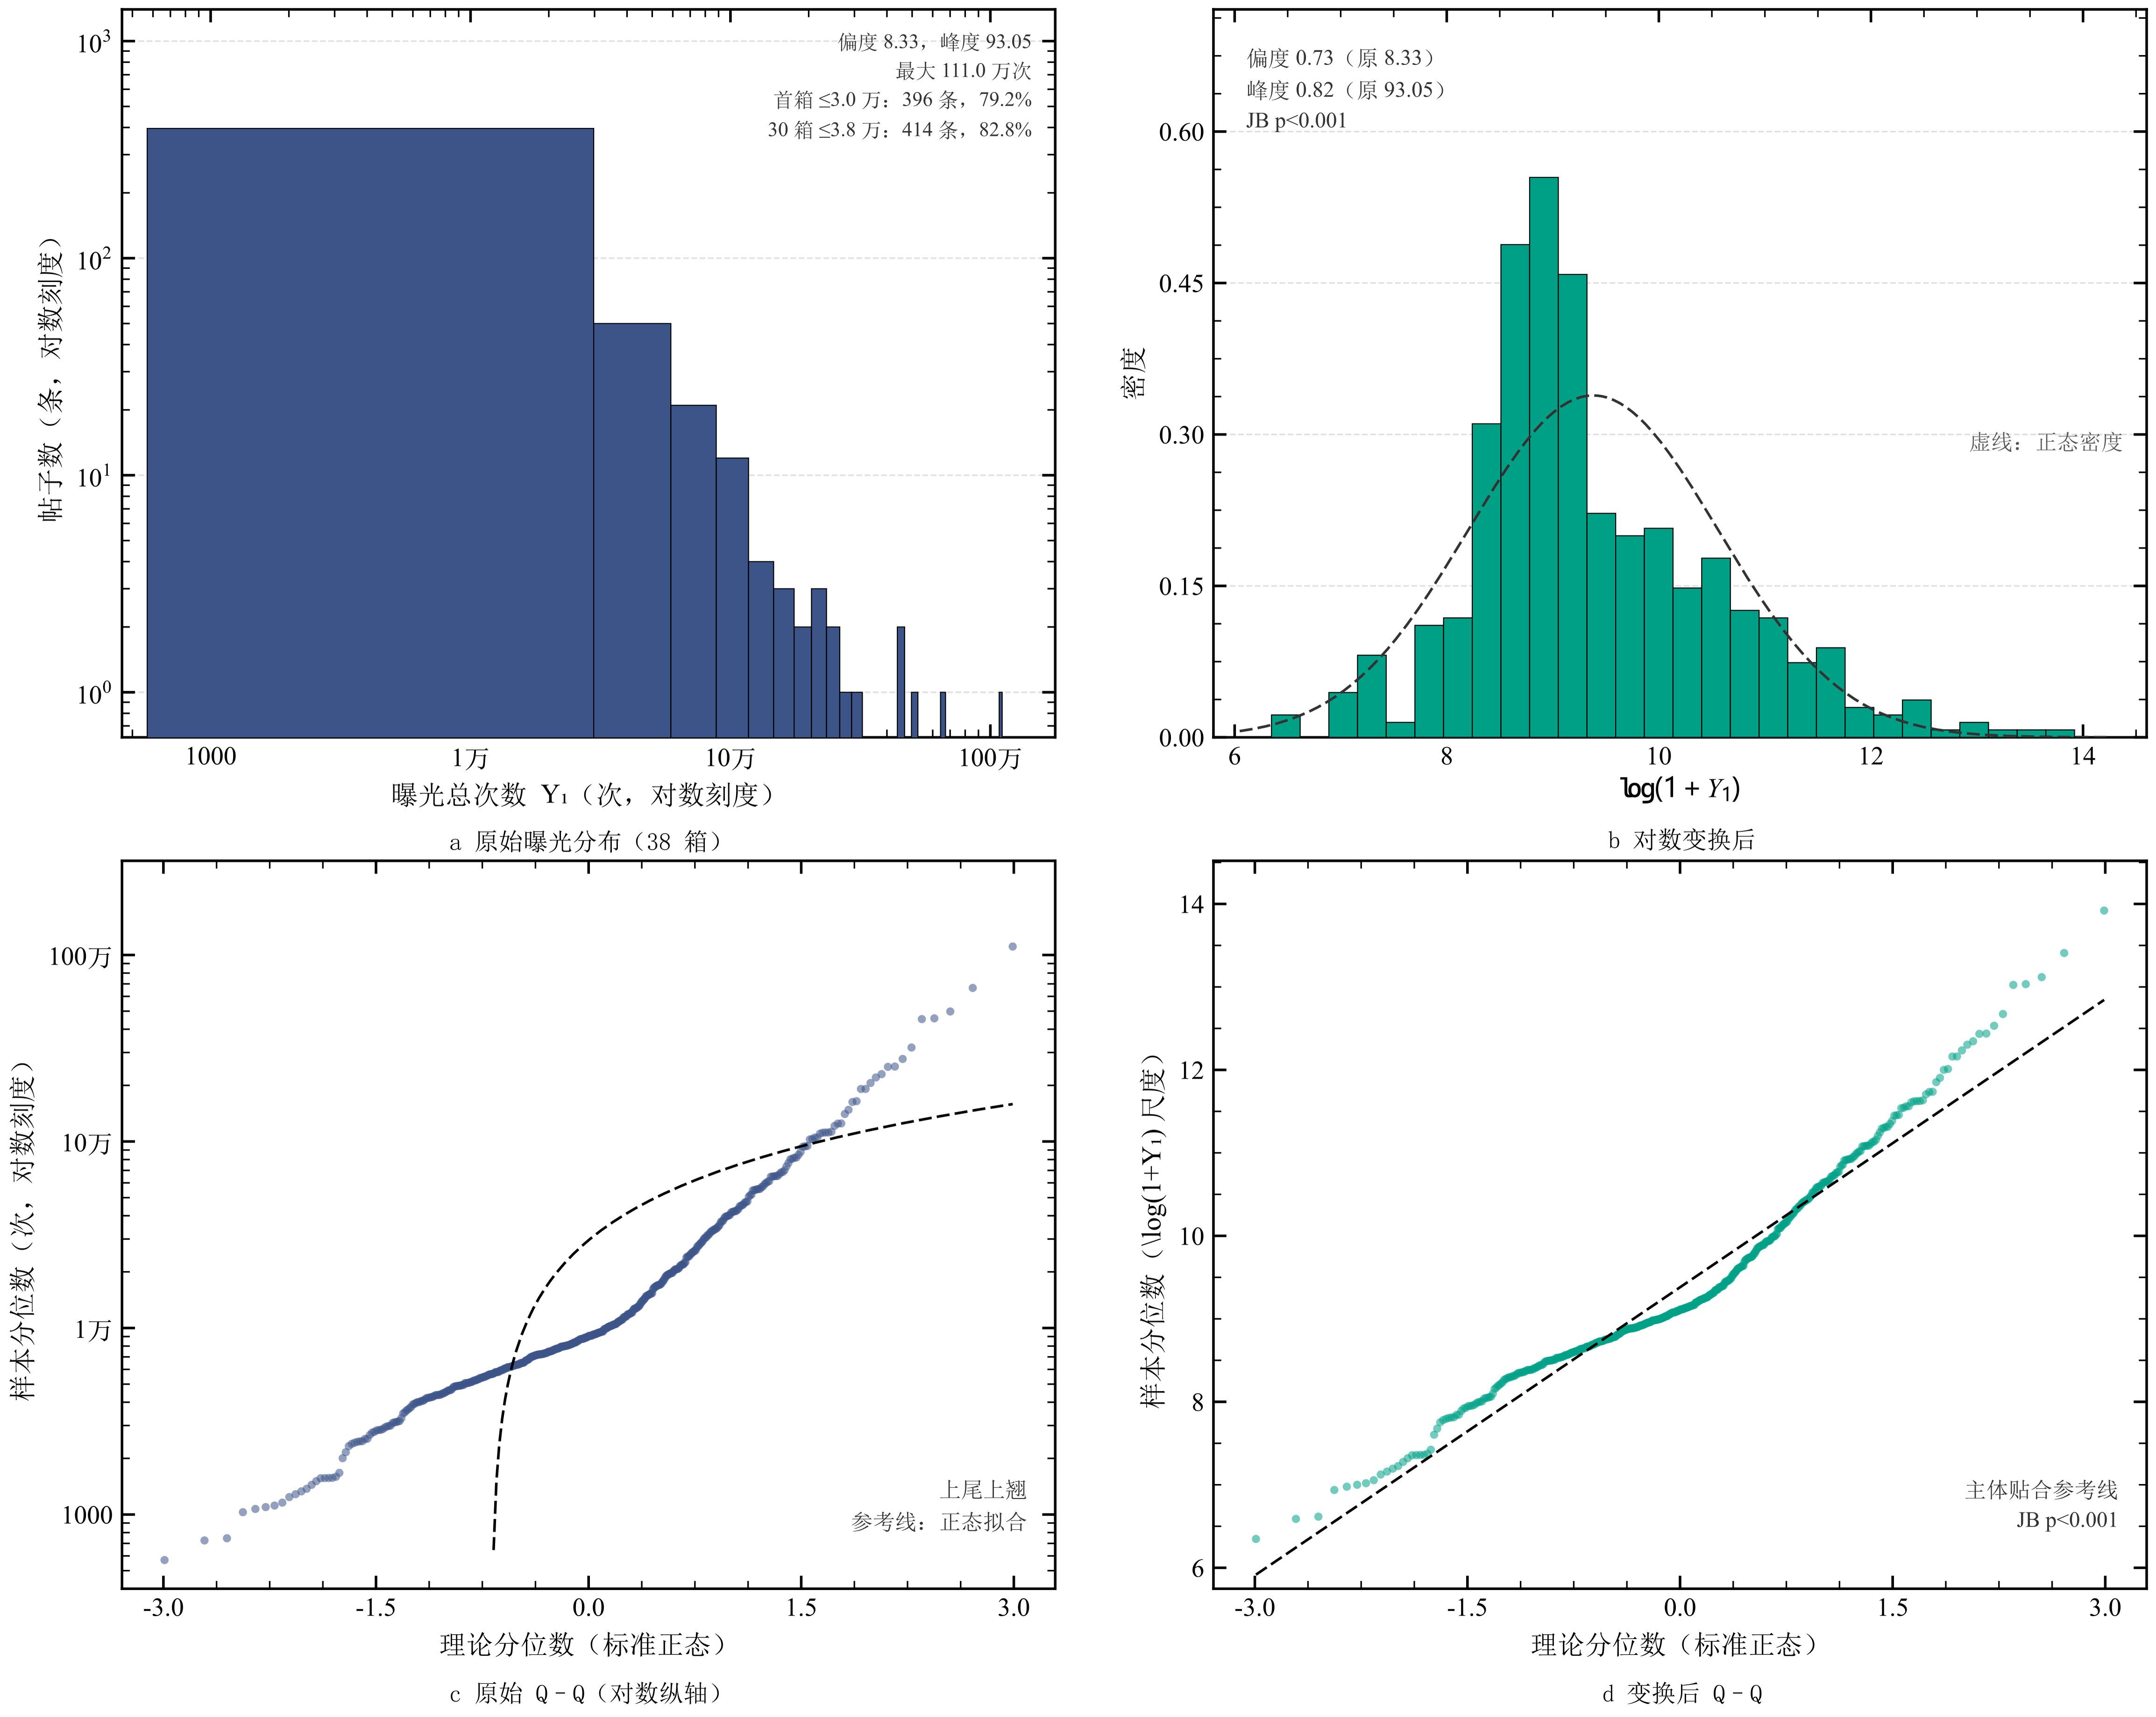
\includegraphics[width=0.70\textwidth]{../求解/问题二/结果/图5_变换前后分布.png}
  \caption{曝光量变换前后的分布与 Q--Q 图}
  \label{fig:q2_trans}
\end{figure}

在完成编码前，图\ref{fig:q2_time}先核对时间变量的经验结构。左上图把逐月发帖量与付费占比放在双轴上：发帖量在 1 月最低（25 条）、10 月最高（60 条），付费占比在 1 月的 16.0\% 与 4 月的 40.0\% 之间波动，既没有单边趋势，也不与发帖量同步。右上图给出逐月平均对数曝光的 95\% 置信带，2 月最高（10.13）、10 月最低（8.83），两月区间不重叠，说明月份既承载账号成长，也混入季节性的内容表现。左下图按星期排列，周四均值最高（9.74）、周日最低（9.06）；右下图按合并后的时段排列，上午最低（9.25）、下午晚间最高（9.50）。不过，星期与时段在控制月份、类型与主题后均不再显著（时段系数的 $p$ 值为 0.150 与 0.638），原始差异主要来自内容构成而非发布时间本身。基于这组证据，月份与星期保留为固定效应，24 小时合并为凌晨、上午、下午晚间三组，以避免稀疏小时带来不稳定估计。

\begin{figure}[ht]
  \centering
  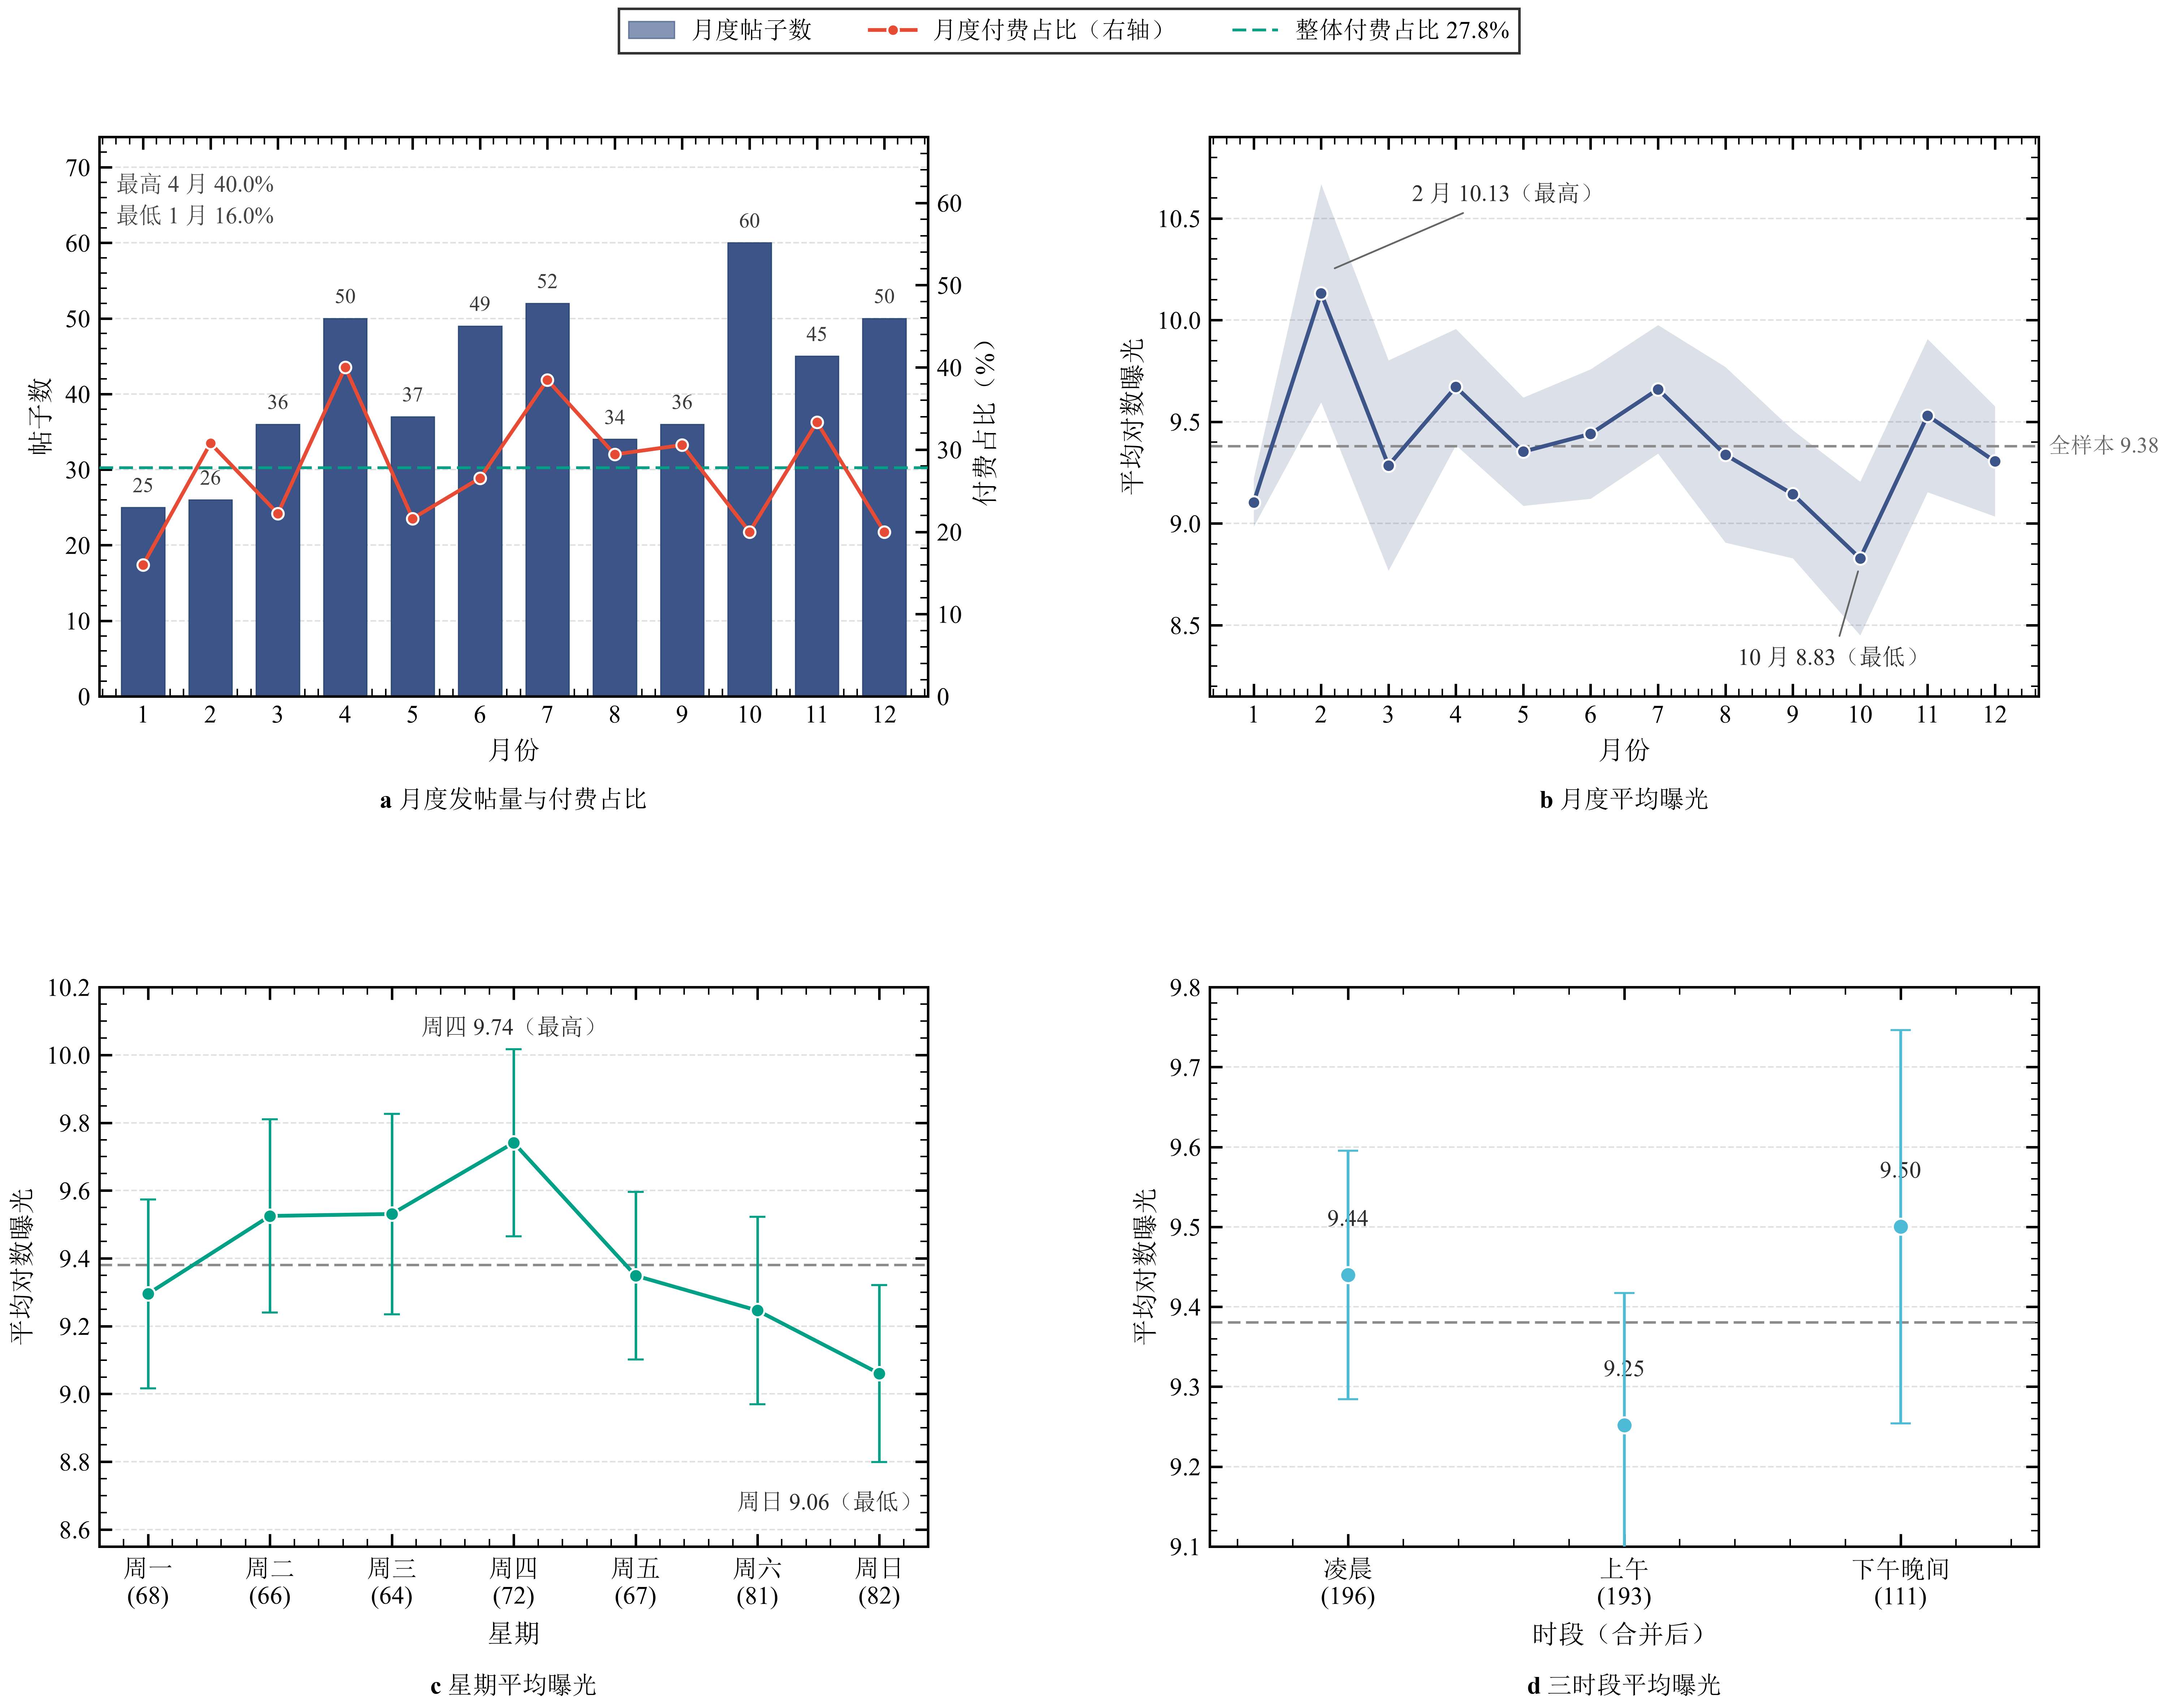
\includegraphics[width=0.70\textwidth]{../求解/临时产物/补充图2_时间结构.png}
  \caption{发帖量、付费占比与曝光的时间结构}
  \label{fig:q2_time}
\end{figure}

缺失处理的敏感性由系数对照给出。众数填补下付费系数为 0.3374、标准误 0.1115、样本量 500；删除缺失行后为 0.3363、标准误 0.1117、样本量 499，两者相差 0.0011，远小于预设的 0.01 阈值。可见填补方案既不改变系数方向，也不改变显著性判断，后续分析使用填补后的 500 条样本。清洗后的数据无缺失、无重复、无越界，类别编码完整，曝光量分布接近对称，可直接供回归建模与效应测算复用。
